\subsubsection{Real Time Values}
Plots the values sampled for a detector in real time. Not all detectors provide both Count Rate and Dose Rate, in such cases the detector is still registered to the plot but noting is shown in LuRaCs spectrum view/tab. The y-axes can be changed from linear to logarithmic scale clicking Mouse-2 on the plot \texttt{Plot Options -> Transforms -> Log Y}.
\begin{figure}[H]
    \centering
    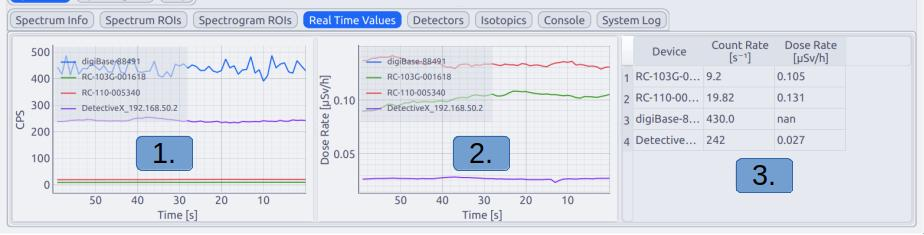
\includegraphics[width = .9\linewidth]{images/interface/real_time_tab.jpg}
    \caption{Real Time Values with four different detectors connected.}
    \label{fig:real_time_values}
    \begin{flushleft}
        \begin{enumerate}
            \item Count Rate plot.
            \item Dose Rate plot, y-axis is always in \unit{\micro\sievert}.
            \item Latest values sampled from the corresponding detector.
        \end{enumerate}
    \end{flushleft}
\end{figure}